\RequirePackage{snapshot}
\documentclass[10pt,a4paper]{ULBreport}
\usepackage[utf8]{inputenc}
\sceau{Images/sceauULB.jpg}
\graphicspath{ {./Images/} }
\usepackage{multirow}
\usepackage{listings}
\usepackage{color} 
\usepackage{setspace} 
\usepackage{amsmath}

\usepackage{pdfpages}
\usepackage{biblatex}
\usepackage{floatrow}
\usepackage{subcaption} 
\usepackage{siunitx}
\usepackage[many]{tcolorbox}
\usepackage{multirow}
\usepackage{soul}
\usepackage[final]{pdfcomment}
\usepackage{listings}
\usepackage[dvipsnames]{xcolor}
\usepackage{fancyvrb}
\usepackage{hyperref}
\usepackage{xstring}
\usepackage{etoolbox}
\usepackage{svg}

\setcounter{chapter}{-1}

% Colors


% BOXES FOR QUESTIONS

\newtcolorbox{questionBox}[2][]{
    fontupper=\bf,
    boxrule=1.5pt,
    colframe= black, % frame color
    fonttitle=\itshape,
    attach boxed title to top left={yshift=-0.3\baselineskip-0.4pt,xshift=2mm},
    title= #2,#1,
    enhanced,
    }

\newtcolorbox{bonusQuestionBox}[2][]{
    fontupper=\bf,
    boxrule=1.5pt,
    colframe= Peach, % frame color
    colback=Apricot,
    coltitle=black,
    fonttitle=\itshape,
    attach boxed title to top left={yshift=-0.3\baselineskip-0.4pt,xshift=2mm},
    boxed title style={colback=BurntOrange},
    title= #2,#1,
    enhanced,
    }





\begin{document} 


	\titleULB{
	title={Report Lab 5 \\ Certificate Authority and NAT},
    studies={IRELE - MA1 Electrical Engineering},
    course ={ELEC-H417},
    author={\textit{Authors :} \\ Amaury ARICO \\ Alexis BOLLENGIER \\ Emmeran COLOT \\Sefa GÖNEN  },
    date={\textbf{Academic year :} \\ 2024 - 2025},
    teacher={\textit{Professor : } \\ Jean-Michel DRICOT \\\textit{Assistant : } \\ Navid LADNER },
    logo={Images/logo-polytech.jpg},
    manyAuthor
	}

\chapter{Mission 0 - Certificate Authority}




\section{Question - Authentication method between PC1 and PC2 before CA}

\begin{questionBox}{Authentication method between PC1 and PC2 before CA}
    Explain the authentication method used in the previous lab. On what assumption does this method works ? Why would a certificate be necessary ? How would the authentication procedure work ?
\end{questionBox}


In the previous lab, we used the \textbf{Pre-Shared Key Authentication} method : a \textbf{secret key} is \textbf{shared} between PC1 and PC2 and is used to authenticate both parties before establishing connection. This method works on the assumption that this key is \textit{kept secret} and \textit{shared in a secure way} but more importantly that PC1 and PC2 \textbf{agreed on the secret key} (so they already met before).

In the case that a connection between two PCs that \textbf{never met}\footnote{so they didn't agree on a secret shared key before they try to contact each other on an untrusted network} must be established, the \textit{private/public key} cryptography is used. In this approach, a certificate is necessary to prove that the public key is actually owned by the right PC. The authentication procedure would be then based on the certificates : the public key of one entity is encrypted within the certificate. Another entity can have this public key if it decrypts the certificate using the \textbf{public key of the certificate authority} (or CA). By trusting the CA, the authentication is validated and the public key can be used to establish connection. This method is based on trust between the receiver/emitter and the CA.

\section{Question - Importance of clock generation in the CA server}

\begin{questionBox}{Importance of clock generation in the CA server}
    Explain the importance of the clock set up in the router.
\end{questionBox}


Every certificate has an \textbf{expiration date}. It is important to set up the clock in the router to be able to check that a certificate isn't expired. The figure \ref{date} shows the expiration date of the CA's self-signed certificate. Having a \textit{local} time on the router different from the one on the other devices of the network could lead to it considering an outdated certificate valid or a valid one out of date, which are situations to avoid.

\begin{figure}[H]
    \centering
    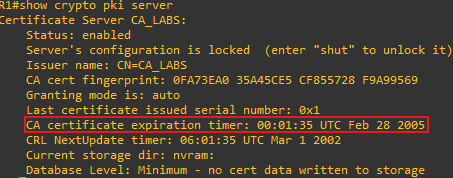
\includegraphics[scale=1]{expdata.png}
    \caption{\texttt{Show crypto pki server} command result for CA router}
    \label{date}
\end{figure}

\section{Question - Certificate}

\begin{questionBox}{Certificate}
    From the router perspective, will you need to accept the certificate ? Capture the certificate exchange in Wireshark.
\end{questionBox}


From the router perspective, we will need to accept or refuse the certificate depending on the authentication of the CA. In fact, the \texttt{crypto pki authenticate TRUSTPOINT\_CA\_LABS} command is used by the router to authenticate the CA : the CA provides the router its self-signed certificate (which contains the public key of the CA). Once the CA has been authenticated, the router can enroll for certificates from the CA. The figure \ref{exchange} shows the certificate exchange.
 
\begin{figure}[H]
    \centering
    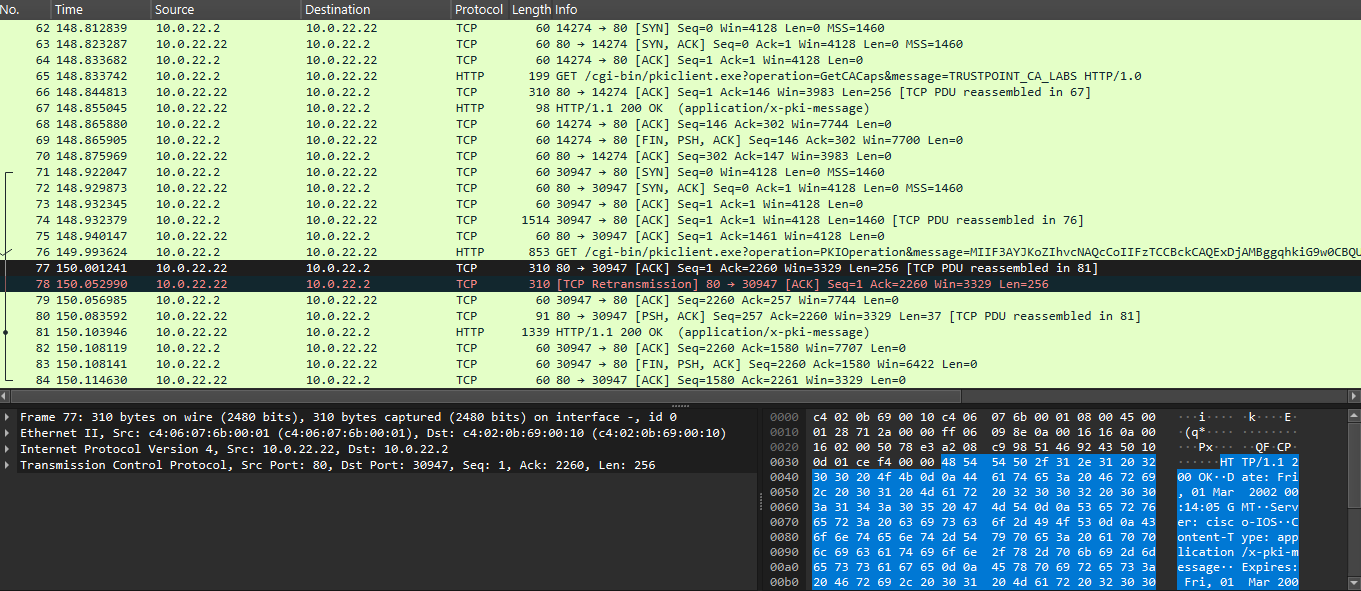
\includegraphics[width=\textwidth]{wiresharkCA.png}
    \caption{Wireshark capture between CA (10.0.22.22) and Router2 (10.0.22.2) - \texttt{crypto pki enroll TRUSTPOINT\_CA\_LABS} command result}
    \label{exchange}
\end{figure}

\chapter{Mission 1 - IPsec \& VPN (again)}

\section{Question - Netmask adaptation}

\begin{questionBox}{Netmask adaptation}
    What should be the netmask to achieve this and why ?
\end{questionBox}


The \textbf{DH} (Diffie-Hellman) \textbf{key exchange protocol} is a protocol used for \textit{securely generating a symmetric cryptographic key over a public channel}\footnote{Source : \url{https://en.wikipedia.org/wiki/Diffie-Hellman_key_exchange}} and works as following :

\begin{itemize}
    \item Both entities agree on public parameters (numbers) that don't have to be kept secret. 
    \item They combine their private key with the public parameters, creating public keys.
    \item Both entities exchange these public keys with each other using the public channel.
    \item They recombine their private key with the received public key.
    \item The result is a secret key that both entities possess and wasn't shared at any point in the public channel.
\end{itemize}

The figures \ref{dhr1} and \ref{dhr2} show the packets used for the protocol.


\begin{figure}[H]
    \centering
    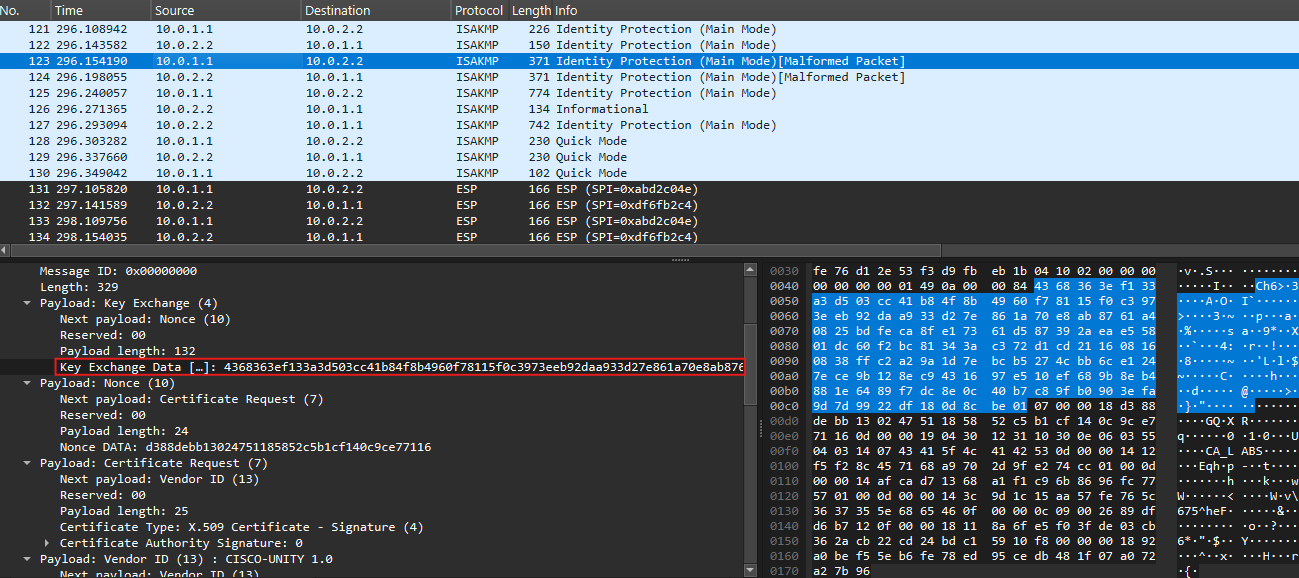
\includegraphics[width=\textwidth]{wiresharkDHR1.png}
    \caption{Wireshark capture between Router1 (10.0.1.1) and Internet - ping from Linux1 to Linux2 command result. Red frame shows the key exchange data from Router1 to Router2 (10.0.1.1)}
    \label{dhr1}
\end{figure}

\begin{figure}[H]
    \centering
    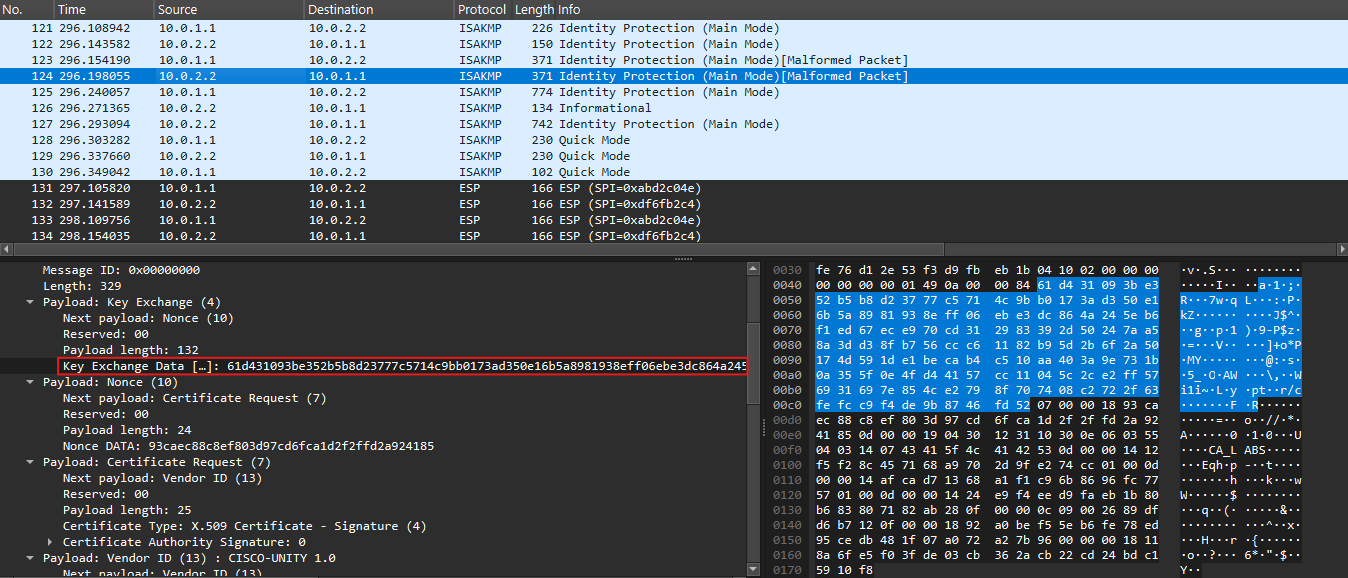
\includegraphics[width=\textwidth]{wiresharkDHR2.png}
    \caption{Wireshark capture between Router1 (10.0.1.1) and Internet - ping from Linux1 to Linux2 command result. Red frame shows the key exchange data from Router2 (10.0.2.2) to Router1 (10.0.1.1)}
    \label{dhr2}
\end{figure}

\chapter{Mission 2 - NAT}



\section{Question - IPv6 compatibility}

\begin{questionBox}{IPv6 compatibility}
    From PC1, ping Router1 and PC2 IPv4 and IPv6 addresses. What is working ? Why ?    
\end{questionBox}


\textbf{NAT} or Network Address Translation is a method used to manipulate the IP address of incoming/outgoing packets in a local network : all devices in a local network \textbf{share just one public IPv4 address}. In other words, the NAT changes the IP address of all packets going out of the local network to one source NAT IP address. The port associated to each packet however depends on the source IP and port. The mapping (public IP + public port $\Leftrightarrow$ local IP + port) is stored in a table, the NAT table, which is used to forward the incoming packets to the intended receiver.

Incoming packets use the source NAT IP address and the new port number as destination address and destination port number. Then the NAT uses its table to translate this port number to the right local IP address and port number. 

\section{Question - How does Traceroute reveal the path between devices ?}

\begin{questionBox}{ How does Traceroute reveal the path between devices ?}
    By analysing carefully your trace command using Wireshark (do not hesitate to capture all the three links), you should be able to understand how it works. Explain in details how the traceroute command works (and interesting observations you can make). What are the layer 3 protocols used and why ?
\end{questionBox}



\begin{enumerate}
    \item There is nothing unusual, the packets are showing PC3's IP address, see figure \ref{nat8080}
    \item In this case, the NAT translates the IP of PC3. That's because we are sending the ping requests with source port 80 of PC3 : we've set up the NAT to translate everything coming from PC3 (192.168.3.3) with port number 80 to 10.0.3.3:1111 NAT IP address and port number, see figure \ref{nat80}.
    \item Again, the NAT translates the IP and port number of the packets to 10.0.3.3:2222 (we've set up it like that in our table).
    \item We get a timeout. PC6 expects a response from PC3 (192.168.3.3:80) but it is the translated packet that it receives (10.0.3.3:1111), see figure \ref{nattime}.
    \item Because we didn't set the port 1111 of PC3 to be translated by the NAT, we get an usual ping command result.
    \item This time, we resolve the timeout we got at the 4th point. The ping requests arrive at the router 3 (10.0.3.3:1111) but because of the NAT, the packets are redirected to PC3. So rather than router 3 responding to the ping, we have in fact packets going from router 3 to PC3. This case is similar to the second point.
    \item This exactly the same case as before but this time, it is PC4 that responds to the ping requests because in the NAT table, the port 2222 is mapped to PC4 (192.168.3.4:80).
\end{enumerate}


\begin{figure}[H]
    \centering
    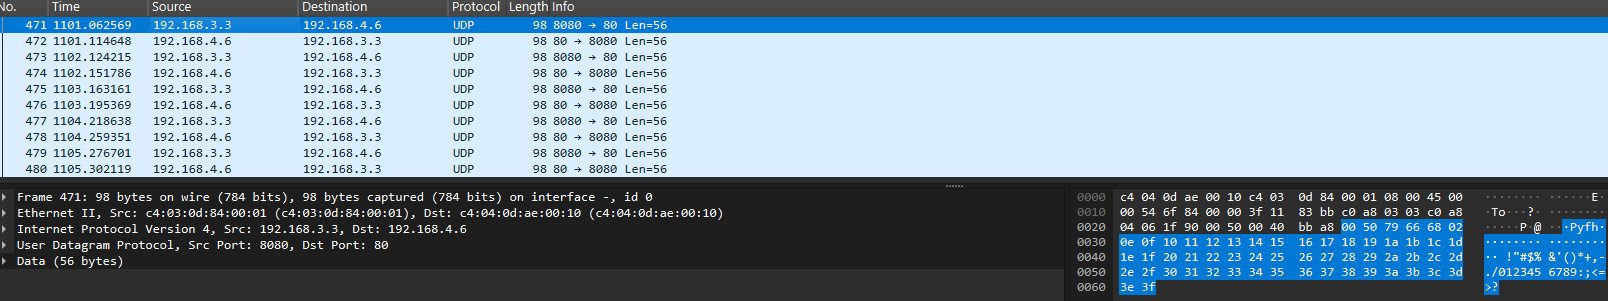
\includegraphics[width=\textwidth]{nat8080.png}
    \caption{Wireshark capture between Router3 (10.0.3.3) and Internet - ping from PC3 port 8080 to PC6 port 80 result}
    \label{nat8080}
\end{figure}

\begin{figure}[H]
    \centering
    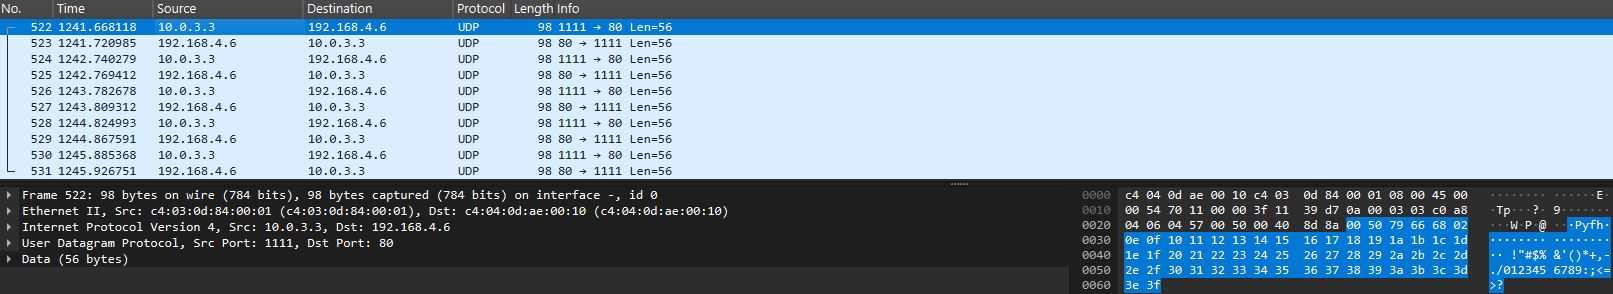
\includegraphics[width=\textwidth]{nat80.png}
    \caption{Wireshark capture between Router3 (10.0.3.3) and Internet - ping from PC3 port 80 to PC6 port 80 result. The NAT translates 192.168.3.3:80 to 10.0.3.3:1111}
    \label{nat80}
\end{figure}

\begin{figure}[H]
    \centering
    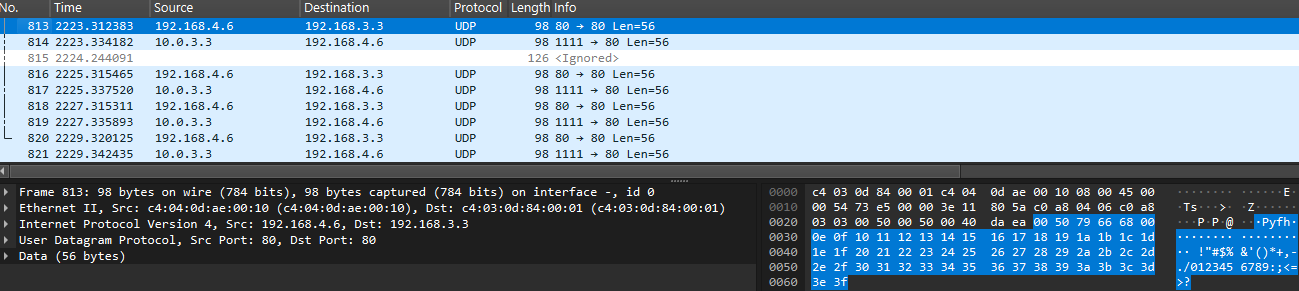
\includegraphics[width=\textwidth]{nattime.png}
    \caption{Wireshark capture between Router3 (10.0.3.3) and Internet - ping from PC6 port 80 to PC3 port 80 result}
    \label{nattime}
\end{figure}

\section{Question - Usage of NAT}

\begin{questionBox}{Usage of NAT}
    Explain how a NAT could be useful in terms of security. Develop some advantages and disadvantages.
\end{questionBox}


NAT offers some security benefits. It masks private/local IP addresses, preventing external access. NAT also helps reducing the number of IPv4 addresses (limited number of possible IPv4 Addresses) and with NAT, it is possible to change addresses in the local network without notifying the outside world as well as changing the ISP without changing addresses of the devices in the local network.

However, NAT does have its disadvantages. First, in order to get a packet from some server, you must connect to it at least once. Also, there is a limited amount of ports (64k ports) and the table needs to be cleaned. Moreover, the NAT adds a bottleneck (all traffic goes through the NAT) and a layer of complexity, which can make troubleshooting more difficult. Some protocols, such as Voice over IP (VoIP) or File Transfer Protocol (FTP), may encounter problems with NAT, requiring adjustments.

\end{document}

% frame.number >= && frame.number <=
% ping ip_address -P 17 -p DSTPORT -s SRCPORT
